\title{Solutions for Homework 3}
\author{Dr. Jordan Hanson - Whittier College Dept. of Physics and Astronomy}
\date{\today}
\documentclass[10pt]{article}
\usepackage[a4paper, total={18cm, 27cm}]{geometry}
\usepackage{graphicx}
\usepackage{amsmath}
\usepackage{tcolorbox}

\def\rcurs{{\mbox{$\resizebox{.16in}{.08in}{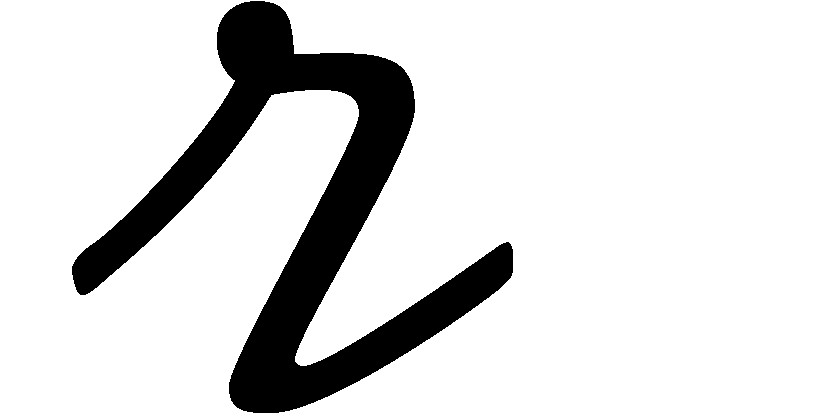
\includegraphics{ScriptR}}$}}}
\def\brcurs{{\mbox{$\resizebox{.16in}{.08in}{
\includegraphics{BoldR}}$}}}
\def\hrcurs{{\mbox{$\hat \rcurs$}}}

\begin{document}
\maketitle

\section{Problem 3.3}

The Laplacian in spherical coordinates, assuming $V(\mathbf{r})$ depends only on $r$, is

\begin{equation}
\frac{1}{r^2}\frac{\partial}{\partial r}\left( r^2 \frac{\partial V}{\partial r}\right) = 0
\end{equation}

\begin{itemize}
\item Multiply both sides by $r$, assuming that $r \neq 0$ (for the Laplacian has a potential singularity there).
\item The quantity $(r^2 dV/dr)$ must be a constant because its derivative is zero.
\item We have
\begin{align}
r^2 \frac{dV}{dr} &= k \\
\frac{dV}{dr} &= \frac{k}{r^2} \\
V(r) &= - \frac{k}{r} + C
\end{align}
Thus the $1/r$ dependence of potential with spherical symmetry is a consequence of Laplace's Equation.  
\end{itemize}

The Laplacian in cylindrical coordinates, assuming $V(\mathbf{r})$ depends only on $s$, is

\begin{equation}
\frac{1}{s}\frac{\partial}{\partial s}\left( s \frac{\partial V}{\partial s}\right) = 0
\end{equation}

Using the same approach as the steps above, we find that $s$ times $dV/ds$ is a constant and that 

\begin{equation}
V(s) = k\ln(s) + C
\end{equation}

Imagine the solution for the potential surrounding a line charge, and notice that it follows this pattern.

\section{Problem 3.5}

\textit{Prove that the field is uniquely determined when the charge density $\rho$ is given and either $V$ or the normal derivative $\partial V/ \partial n$ is specified on each boundary surface.  Do not assume the boundaries are conductors, or that $V$ is constant over any given surface.} \\ \\

This proof follows closely the one on pp. 121-123, with one key difference.  Start by assuming there are two solutions for the field within the volume $\mathcal{V}$ where we find $\rho$.  There is only one $\rho$, but there could be many objects (conductors or otherwise) within the volume, and one global surface containing them all.  The two solutions follow the original reasoning:

\begin{align}
\nabla \cdot \mathbf{E}_1 &= - \frac{\rho}{\epsilon_0} \\
\nabla \cdot \mathbf{E}_2 &= - \frac{\rho}{\epsilon_0} \\
\mathbf{E}_3 &= \mathbf{E}_2 - \mathbf{E}_1 \\
\nabla \cdot \mathbf{E}_3 &= 0 \\
\oint \mathbf{E}_3 \cdot d\mathbf{a} &= 0 ~~ (all ~~ surfaces) \\
\mathbf{E}_3 &= -\nabla V_3 \\
\nabla \cdot (V_3 \mathbf{E}_3) &= V_3 (\nabla \cdot \mathbf{E}_3) + \mathbf{E}_3 (\nabla V_3) = 0 - \mathbf{E}_3 \cdot \mathbf{E}_3 = - E_3^2
\end{align}

Integrate the final line with respect to volume, over $\mathcal{V}$:

\begin{equation}
\int_\mathcal{V} \nabla \cdot (V_3 \mathbf{E}_3) d\tau = -\int E_3^2 d\tau
\end{equation}

Use the divergence theorem on the left-hand side:

\begin{equation}
\oint V_3 \mathbf{E}_3 \cdot d\mathbf{a} = -\int E_3^2 d\tau
\end{equation}

The integrand on the left hand is zero if:

\begin{itemize}
\item The potentials $V_1$ and $V_2$ are specified on each surface.  Then, $V_3$ over each and every surface, and the integrand is zero.
\item The normal derivatives $\partial V_1 / \partial n$ and $\partial V_2 / \partial n$ are specified.  Then, $\partial V_3 / \partial n = -E_{3,\perp} = 0$, and the integrand is zero.
\end{itemize}

Thus, either way, the integrand is zero and 

\begin{equation}
\int E_3^2 d\tau = 0
\end{equation}

That means that $E_3 = 0$, and $\mathbf{E}_2 = \mathbf{E}_1$.  The field is unique.

\section{Problem 3.6}

\textit{A more elegant proof of the second uniqueness theorem uses Green's identity (Problem 1.16c), with $T = U = V$.  Supply the details.} \\ \\

And ... go!

\begin{align}
\int_\mathcal{V} (V_3 \nabla^2 V_3 + \nabla V_3 \cdot \nabla V_3) d\tau &= \oint (V_3 \nabla V_3) \cdot d\mathbf{a} \\
\int_\mathcal{V} (0 + \nabla V_3 \cdot \nabla V_3) d\tau &= - \oint (V_3 \mathbf{E}_3) \cdot d\mathbf{a} \\
- \int_\mathcal{V} E_3^2 d\tau &= - \oint (V_3 \mathbf{E}_3) \cdot d\mathbf{a} \\
\int_\mathcal{V} E_3^2 d\tau &= \oint (V_3 \mathbf{E}_3) \cdot d\mathbf{a}
\end{align}
Using the same logic as the prior exercises completes the proof.

\section{Problem 3.13}

\textit{Find the potential in the infinite slot of Ex. 3.3 if the boundary at $x=0$ consists of two metal strips: one, from $y=0$ to $y=a/2$, is held at a positive constant potential $V_0$, and the other, from $y=a/2$ to $y=a$, is held at a negative constant potential $-V_0$.} \\ \\

Using Ex. 3.3, one can arrive at

\begin{align}
V(x,y) &= \sum_{n = 1}^{\infty} C_n e^{-n \pi x / a} \sin(n \pi y / a) \\
C_n &= \frac{2}{a}\int_0^a V_0(y) \sin(n \pi y / a) dy 
\end{align}

The Fourier coefficient is found by applying the boundary condition:

\begin{equation}
C_n = \frac{2V_0}{a} \left( \int_0^{a/2} \sin(n\pi y/a) dy - \int_{a/2}^{a} \sin(n\pi y/a) dy\right) = \frac{2 V_0}{n\pi}(1+(-1)^n - 2\cos(n\pi/2))
\end{equation}

How do we generalize the result into a sum of solutions?  Notice that the coefficient is zero if (a) $n$ is odd, or (b) $n$ is a multiple of 4.  Otherwise, it turns into $4$.  Thus:

\begin{equation}
C_n = \frac{8V_0}{n\pi}, ~~ n = (4j+2), ~ j = 0,1,2, ...
\end{equation}

The solutions can be gathered into the series above like so:

\begin{equation}
V(x,y) = \frac{8V_0}{\pi}\sum_{j=0}^{\infty} \frac{e^{-(4j+2)\pi x / a} \sin((4j+2) \pi y/a)}{4j+2}
\end{equation}

\section{Problem 3.14}

\textit{For the infinite slot (Ex. 3.3), determine the charge density $\sigma(y)$ on the strip at $x=0$, assuming it is a conductor at constant potential $V_0$.} \\ \\

Note that the exercises states that the surface is a \textbf{conductor.}  This means that

\begin{equation}
\frac{\partial V}{\partial n} = -\frac{\sigma}{\epsilon_0}
\end{equation}

(The field is zero on the other side of the conductor.  Otherwise, there would be a factor of two).  Recall the result $V(x,y)$ for the potential:

\begin{equation}
V(x,y) = \frac{4V_0}{\pi} \sum_{n = 1,3,5, ...} \frac{1}{n}e^{-n\pi x/a}\sin(n\pi y/a)
\end{equation}

Rearrange the above boundary condtion to obtain $\sigma(y)$:

\begin{align}
\sigma(y) &= -\epsilon_0 \left.\frac{\partial V}{\partial x}\right|_{x=0} \\
\sigma(y) &= \frac{4\epsilon_0 V_0}{a}\sum_{n=0}^{\infty} \sin((2n+1)\pi y/a)
\end{align}

Notice that:
\begin{itemize}
\item The charge density has the right units, because $a$ has units of length.
\item If $y=0$ or $y=a$, the charge density goes to zero.
\end{itemize}

\section{Problem 3.15}

\textit{A rectangular pipe, running parallel to the z-axis (from $-\infty$ to $\infty$), has three grounded metal sides, at $y=0$, $y=a$, and $x=0$.  The fourth side, at $x=b$, is maintained at a specified potential $V_0(y)$.  (a) Develop a general formula for the potential inside the pipe.  (b) Find the potential explicitly, for the case $V_0(y) = V_0$, a constant.} \\ \\
Using the separation of variables technique to solve Laplace's Equation leads to

\begin{align}
\frac{1}{X(x)}\frac{d^2X}{dx^2} &= \pm k^2 \\
\frac{1}{Y(y)}\frac{d^2Y}{dy^2} &= \pm k^2
\end{align}

The solutions are either positive and negative exponentials for $+k^2$, or sinusoids for $-k^2$ on the right-hand side.  If we select sinusoids for the $y$-coordinate, then eventually the boundary conditions will yield a familiar Fourier series to match $V_0(y)$.  The form of the solution is

\begin{equation}
V(x,y) = \left( A\sin(ky) + B\cos(ky) \right)\left( C e^{kx} + D e^{-kx} \right)
\end{equation}

Here are the boundary conditions:

\begin{itemize}
\item $V = 0$ if $y=0$ and $y=a$
\item $V = 0$ if $x=0$
\item $V = V_0(y)$ if $x = b$
\end{itemize}

To match the boundary conditions, take $A=0$, $B\neq 0$ but with $k=n\pi/a$, and $C=-D$.  There is one overall coefficient left, and the specific solution is that coefficient times hyperbolic sine, times sine.  The general solution is the sum of all specific solutions:

\begin{equation}
V(x,y) = \sum_{n=0}^{\infty} C_n \sin(n\pi y/a) \sinh(n\pi x/a)
\end{equation}

Using \textbf{Fourier's Trick} to find $C_n$ gives

\begin{equation}
C_n = \frac{2}{a \sinh(n \pi b/a)}\int_0^{a} V_0(y) \sin(n\pi y/a) dy
\end{equation}

If $V_0(y) = V_0$, then the $C_n$ becomes, with $n = 1,3,5,...$

\begin{equation}
C_n = \frac{4V_0}{n\pi\sinh(n\pi)}
\end{equation}

The general sum of solutions is

\begin{equation}
V(x,y) = \frac{4V_0}{\pi}\sum_{n=0}^{\infty} \frac{\sin((2n+1)\pi y/a)\sinh((2n+1))\pi x/a)}{(2n+1)\sinh(n\pi b/a)}
\end{equation}

\section{Problem 3.16}

\textit{A cubical box (sides of length $a$) consists of five metal plates, which are welded together and grounded.  The top is made of a separate sheet of metal, insulated from the others, and held at a constant potential $V_0$.  Find the potential inside the box.} \\ \\

The six boundary conditions correspond to the six sides, and suggest sinusoids in the $x$ and $y$ coordinates and exponentials in the $z$ coordinate.  These three differential equations describe the separable solutions:

\begin{align}
\frac{1}{X(x)}\frac{d^2X}{dx^2} &= -k^2 \\
\frac{1}{Y(y)}\frac{d^2Y}{dy^2} &= -l^2 \\
\frac{1}{Z(z)}\frac{d^2Z}{dz^2} &= (k^2+l^2)
\end{align}

Thus, the sum of the solutions is zero and Lacplace's Equation is satisfied.  The specific solutions are 

\begin{align}
X(x) &= A\cos(kx) + B\sin(ky) \\
X(x) &= C\cos(lx) + D\sin(ly) \\
Z(z) &= E\exp(-z\sqrt{k^2+l^2}) + F\exp(z\sqrt{k^2+l^2})
\end{align}

The boundary conditions require $A = C = 0$, and $B\neq 0, ~ D\neq 0$ with $k=n\pi/a$ and $l=m\pi/a$, and $E + F = 0$.  The general solution is 

\begin{equation}
V(x,y,z) = \sum_{n} \sum_{m} C_{n,m} \sin(n\pi x/a)\sin(m\pi y/a)\sinh(\pi\sqrt{n^2+m^2}z/a)
\end{equation}

The final boundary condition gives

\begin{equation}
V_0 = \sum_{n} \sum_{m} C_{n,m} \sin(n\pi x/a)\sin(m\pi y/a)\sinh(\pi\sqrt{n^2+m^2})
\end{equation}

Perform \textbf{Fourier's Trick} twice to obtain an expression for $C_{n,m}$:

\begin{equation}
C_{n,m} \sinh(\pi\sqrt{n^2+m^2}) = \left(\frac{2}{a}\right)^2 V_0 \int_0^a\int_0^a \sin(n\pi x/a)\sin(m\pi y/a) dx dy = \frac{16 V_0}{\pi^2 n m}, ~~ n,m~ odd
\end{equation}

Solve for $C_{n,m}$ and reinsert into $V(x,y,z)$ to obtain

\begin{equation}
V(x,y,z) = \frac{16V_0}{\pi^2}\sum_{n~odd}\sum_{m~odd} \frac{\sin(n\pi x/a)\sin(m\pi y/a)}{nm}\frac{\sinh(\pi \sqrt{n^2 + m^2} z/a)}{\sinh(\pi \sqrt{n^2 + m^2})}
\end{equation}

\textbf{Bonus point:} show that the result of this sum is $V_0/6$ for $x = y = z = a/2$.  (Requires numerical evaluation).

\section{Problem 3.19}

\textit{The potential at the surface of a sphere of radius $R$ is given by $V_0 = k\cos 3\theta$, where $k$ is a constant.  Find the potential inside and outside the sphere, as well as the surface charge density $\sigma(\theta)$ on the sphere.  (Assume there is no charge inside or outside the sphere).} \\ \\

After playing around with trigonometric formulas and Legendre polynomials, one can show that

\begin{equation}
V_0 = \frac{k}{5}(8P_3(\cos\theta) - 3P_1(\cos\theta))
\end{equation}

Following the separation of variables procedure, the solutions for inside and outside the spherical shell are

\begin{align}
V(r,\theta) &= \sum_{l=0}^{\infty} A_l r^l P_l(\cos\theta), ~~ r\leq R \\
V(r,\theta) &= \sum_{l=0}^{\infty} B_l r^{-(l+1)} P_l(\cos\theta), ~~ r\geq R
\end{align}

The solutions must be continuous at the boundary, so $V_{in}(R,\theta) = V_{out}(R,\theta)$.  According to Eq. 3.69 of the text,

\begin{equation}
A_l = \frac{2l+1}{2R^l}\int_0^\pi V_0(\theta)P_k(\cos\theta)\sin\theta d\theta
\end{equation}

Since $V_0(\theta)$ contains only two distinct Legendre polynomials, there are only two $A_l$ values that are not zero: $k = 1$, and $k = 3$.  The results are

\begin{itemize}
\item $A_1 = -3k/5R$
\item $A_3 = 8k/5R^3$
\end{itemize}

The general solution within the spherical shell is then

\begin{equation}
V_{\rm in}(r,\theta) = -\frac{3k}{5R} r P_1(\cos\theta) + \frac{8k}{5R^3} r^3 P_3(\cos\theta)
\end{equation}

Now consider the region outside the sphere, with $r \geq R$.  We know that $B_1 = A_1 R^{2l+1}$ because the potential must be continuous at $r = R$.  This means that the only non-zero $B$ coefficients are $B_1$ and $B_3$:

\begin{itemize}
\item $B_1 = -3k R^2/5$
\item $B_3 = 8k R^4/5$
\end{itemize}

The general solution outside the spherical shell is then

\begin{equation}
V_{\rm out}(r,\theta) = -\frac{3kR^2}{5r^2} P_1(\cos\theta) + \frac{8k R^4}{5r^4} P_3(\cos\theta)
\end{equation}

Equation 3.83 of the text gives $\sigma(\theta)$ at $r = R$, which is just forcing the discontinuity in the normal derivative of the potential at $r = R$ to be proportional to $\sigma$:

\begin{equation}
\sigma(\theta)= \epsilon_0 [3 A_1 P_1 + 7 A_3 R^2 P_3]
\end{equation}

\section{Problem 3.22}

\textit{In Problem 2.25, you found the potential on the axis of a uniformly charged disk: $V(r,0) = \sigma/(2\epsilon_0) \left( \sqrt{r^2 + R^2} - r\right)$.}

\begin{itemize}
\item (a) \textit{Use this, together with the fact that $P_l(1) = 1$, to evaluate the first three terms in the Legendre expansion (Eq. 3.72) for the potential of the disk at points off the axis, assuming $r > R$.} \\ \\
As usual, the general solution is a sum of Legendre polynomials like:

\begin{equation}
V(r,\theta) = \sum_{l=0}^{\infty} \frac{B_l}{r^{(l+1)}} P_l(\cos\theta)
\end{equation}

The boundary condition is our solution on-axis:

\begin{equation}
V(r,0) = \sum_{l=0}^{\infty} \frac{B_l}{r^{(l+1)}} P_l(1) = \sum_{l=0}^{\infty} \frac{B_l}{r^{(l+1)}} = \frac{\sigma}{2\epsilon_0} \left( \sqrt{r^2 + R^2} - r\right)
\end{equation}

What we see on the left side is a power series in $r$, and on the right is a function of $r$.  The idea is to expand the right side in a series in $r$, and match like powers of $r$ on both sides.  Note that

\begin{equation}
\sqrt{r^2 + R^2} = r\left( 1 + \frac{1}{2}\left(\frac{R}{r}\right)^2 - \frac{1}{8}\left(\frac{R}{r}\right)^4\right)
\end{equation}

Inserting this result into the equation from the boundary condition eventually leads to
\begin{enumerate}
\item $B_0 = \frac{\sigma R^2}{4\epsilon_0}$
\item $B_1 = 0$
\item $B_2 = \frac{\sigma R^4}{16 \epsilon_0}$
\end{enumerate}

Apparently the only Legendre polynomials that turn up in the first three terms are $P_0$ and $P_2$, which makes sense because the charge distribution has even symmetry in $\cos\theta$.  The solution is
\begin{equation}
V(r,\theta) \approx \frac{\sigma R^2}{4\epsilon_0}\left( \frac{1}{r} - \frac{R^2}{4r^3}P_2(\cos\theta)\right)
\end{equation}

\item \textit{Find the potential for $r < R$ by the same method, using Eq. 3.66.  Note: Break the interior region into the two hemispheres.  Do not assume identical coefficients for above and below the disk.}

The pattern of reasoning follows the same process as above, but using Eq. 3.66 of the text, and the same boundary condition.  Here we quote the results for above and below the disk:

\begin{align}
V_{\rm above}(r,\theta) &\approx \frac{\sigma}{2\epsilon_0} \left( R - rP_1(\cos\theta) + \frac{r^2}{2R}P_2(\cos\theta) \right) \\
V_{\rm below}(r,\theta) &\approx \frac{\sigma}{2\epsilon_0} \left( R + rP_1(\cos\theta) + \frac{r^2}{2R}P_2(\cos\theta) \right)
\end{align}
\end{itemize}


\section{Problem 3.24}

\textit{Solve Laplace's equation by separation of variables in cylindrical coordinates, assuming there is no dependence on z (cylindrical symmetry).  Make sure you find all solutions to the radial equation. In particular, your result must accommodate the case of an infinite line charge.} \\ \\

Laplace's equation in cylindrical coordinates, with the z-dependence eliminated gives

\begin{equation}
\frac{1}{s}\frac{\partial}{\partial s}\left( s \frac{\partial V}{\partial s} \right) + \frac{1}{s^2} \left( \frac{\partial^2 V}{\partial \phi^2} \right) = 0
\end{equation}

Much like Cartesian coordinates, the solutions separate.  Consider the $\phi$ solutions first, and assume the constant is negative:

\begin{equation}
\frac{1}{\Phi} \frac{d^2\Phi(\phi)}{d\phi^2} = -k^2
\end{equation}

This produces sinusoidal solutions, and they periodic like $\Phi(\phi) = \Phi(\phi+2\pi)$, so $k$ is an integer.  That means the other solutions, for $S(s)$, have to come from

\begin{equation}
\frac{s}{S(s)}\frac{d}{d s}\left( s \frac{d S(s)}{d s} \right) = k^2
\end{equation}

With the differentiating and dividing/mulitplying by $s$, a good guess is $S(s) = s^n$, provided we have the right $n$ (which is an integer).  Plugging in gives the result $n = \pm k$.  We have

\begin{equation}
S(s) = C s^k + D s^{-k}
\end{equation}

If, however, $k = 0$, then $S = const$, and there should be two solutions (the equation we're solving is second-order).  Turns out, we already addressed this in Problem 3.3.  The result was

\begin{equation}
S(s) = C \ln(s) + D
\end{equation}

Considering $k = 0$ for $\Phi(\phi)$ yields something that does not have periodic boundary conditions.  The most general way to summarize the separable solution is 

\begin{equation}
V(s,\phi) = a_0 + b_0\ln(s) + \sum_{k=1}^{\infty}\left[ s^k(a_k\cos(k\phi) + b_k\sin(k\phi)) + s^{-k}(c_k\cos(k\phi) + d_k\sin(k\phi)) \right] \label{eq:gen}
\end{equation}

The infinite line charge does go like $V(s) \approx \ln(s)$.


\section{Problem 3.26}

\textit{Charge density $\sigma(\phi) = a \sin(5\phi)$, where $a$ is a constant.  This charge density is glued over the surface of an infinite cylinder of radius $R$.  Find the potential inside and outside the cylinder.  Use the tools from the prior problem.} \\ \\

Consider \textbf{inside} the cylinder first.  Cutting away the parts of the general solution (Eq. \ref{eq:gen}) that blow up at $s = 0$:

\begin{equation}
V_{\rm in} (s,\phi) = a_0 + \sum_{k=1}^{\infty} s^k (a_k \cos(k\phi)+ b_k \sin(k\phi) )
\end{equation}

Consider now the region \textbf{outside} the cylinder.  Cutting away the parts of the general solution that blow up at $s \to \infty$:

\begin{equation}
V_{\rm out} (s,\phi) = a'_0 + \sum_{k=1}^{\infty} \frac{1}{s^k} (c_k \cos(k\phi)+ d_k \sin(k\phi) )
\end{equation}

The way to obtain potential from $\sigma$ is to assert that the discontinuity in the normal derivative of potential is equal to $\sigma$:

\begin{equation}
\sigma = -\epsilon_0 \left.\left( \frac{\partial V_{\rm out}}{\partial n} - \frac{\partial V_{\rm in}}{\partial n}\right)\right|_{s = R}
\end{equation}

Putting all of this together, by differentiating with respect to $s$ and setting $s = R$, and equating to $\sigma = a\sin(5\phi)$, shows that $k = 5$ with all other terms in the sum vanishing.  This removes $a_k$ and $c_k$ from the game, but $b_5$ and $d_5$ remain and are related.  To solve for them, we need $V_{\rm in}(R,\phi) = V_{\rm out}(R,\phi)$.  Thus, there are two equations with two unknowns $(b_5,d_5)$.  Once these are obtained, we find

\begin{align}
V(s,\phi) &= \frac{a\sin 5\phi}{10\epsilon_0}\frac{s^5}{R^4}, ~~ s \leq R \\
V(s,\phi) &= \frac{a\sin 5\phi}{10\epsilon_0}\frac{R^6}{s^5}, ~~ s \geq R
\end{align}

These solutions are just power laws in $s$ times sinusoids in $\phi$, with no local minima or maxima.

\end{document}
